\documentclass{article}
\usepackage[margin=1in]{geometry}
\usepackage{amsmath}
\usepackage{graphicx}
\usepackage{siunitx}
\usepackage{listings}
\usepackage{xcolor}
\usepackage{booktabs}
\usepackage{hyperref}
\definecolor{mygreen}{rgb}{0,0.6,0}
\definecolor{mygray}{rgb}{0.5,0.5,0.5}
\definecolor{mymauve}{rgb}{0.58,0,0.82}

\lstset{ %
  backgroundcolor=\color{white},   % choose the background color; you must add \usepackage{color} or \usepackage{xcolor}
  basicstyle=\scriptsize\ttfamily,    % the size of the fonts that are used for the code
  breakatwhitespace=false,         % sets if automatic breaks should only happen at whitespace
  breaklines=true,                 % sets automatic line breaking
  captionpos=b,                    % sets the caption-position to bottom
  commentstyle=\color{mygreen},    % comment style
  deletekeywords={},            % if you want to delete keywords from the given language
  escapeinside={\%*}{*)},          % if you want to add LaTeX within your code
  extendedchars=true,              % lets you use non-ASCII characters; for 8-bits encodings only, does not work with UTF-8
  frame=shadowbox,                    % adds a frame around the code
%  framexleftmarign=5mm,
  xleftmargin=10pt,
  xrightmargin=10pt,
  rulesepcolor=\color{gray},
  keywordstyle=\color{blue},       % keyword style
  language=Octave,                 % the language of the code
  morekeywords={*,...,fit,predint,export\_fig},            % if you want to add more keywords to the set
%  numbers=left,                    % where to put the line-numbers; possible values are (none, left, right)
  numbers=none,
  numbersep=5pt,                   % how far the line-numbers are from the code
  numberstyle=\tiny\color{mygray}, % the style that is used for the line-numbers
  rulecolor=\color{black},         % if not set, the frame-color may be changed on line-breaks within not-black text (e.g. comments (green here))
  showspaces=false,                % show spaces everywhere adding particular underscores; it overrides 'showstringspaces'
  showstringspaces=false,          % underline spaces within strings only
  showtabs=false,                  % show tabs within strings adding particular underscores
  stepnumber=1,                    % the step between two line-numbers. If it's 1, each line will be numbered
  stringstyle=\color{mymauve},     % string literal style
  tabsize=4,                       % sets default tabsize to 4 spaces
  caption=\lstname                   % show the filename of files included with \lstinputlisting; also try caption instead of title
}


\title{1.723 Final}
\author{Sachith  Dunatunga}

\begin{document}
\newcommand{\deriv}[2]{\frac{\partial #1}{ \partial #2}}
\newcommand{\nderiv}[3]{\frac{\partial^{#3} #1}{ \partial #2^{#3}}}
\newcommand{\dx}[1]{\deriv{#1}{x}}
\newcommand{\taylorexpf}[3]{#1_{#2} + \left(#3 \right) \dx{#1}\biggr\rvert_{#2} + \frac{1}{2}\left(#3 \right)^2 \nderiv{#1}{x}{2}\biggr\rvert_{#2} + \frac{1}{6}\left(#3 \right)^3\nderiv{#1}{x}{3}\biggr\rvert_{#2} + \frac{1}{24}\left(#3 \right)^4\nderiv{#1}{x}{4}\biggr\rvert_{#2} + O(h^5)}
\maketitle

\section{Problem 1}
\subsection{Part 1}
Since we know $\nabla^2 \Psi = - \omega$, we can write
\begin{align}
    \nabla^2 (\Psi_0 + \tilde{\Psi}) &= -\omega \\
    \nabla^2 \Psi_0 + \nabla^2 \tilde{\Psi} &= -\omega.
\end{align}
However, we know that for this problem $\Psi_0 = y$, since $\mathbf{u}_0 = {1, 0}$.
Therefore, the relationship is given by
\begin{align}
    \nabla^2 y + \nabla^2 \tilde{\Psi} &= -\omega \\
    \nabla^2 \tilde{\Psi} &= -\omega.
\end{align}

In Fourier space, derivatives are taken by multiplying by the wavenumber times the imaginary unit.
Thus, if the fourier transform of $\tilde{\Psi}$ is written as $\hat{\tilde{\Psi}}$, the fourier transform of $\nabla^2 \tilde{\Psi}$ is given by
\begin{align}
    \nabla^2 \tilde{\Psi} &= \nderiv{\tilde{\Psi}}{x}{2} + \nderiv{\tilde{\Psi}}{y}{2} \\
\implies \widehat{\nabla^2 \tilde{\Psi}} &= (ik_x)^2 \hat{\tilde{\Psi}} + (ik_y)^2 \hat{\tilde{\Psi}}\\
    \widehat{\nabla^2 \tilde{\Psi}} &= -(k^2_x + k^2_y) \hat{\tilde{\Psi}}.
\end{align}

Since at zero frequency in both x and y we have $\exp(0) = 1$, the fourier transform turns into the average value of the signal.
In this case, since we only care about derivatives of the stream function $\Psi$, this constant is `free' and will not affect the results.

\subsection{Part 2}
From the previous problem we have
\begin{align}
    \widehat{\nabla^2 \tilde{\Psi}} &= -(k^2_x + k^2_y) \hat{\tilde{\Psi}}.
\end{align}
We can write the fourier transform of the equation
\begin{align}
    \nabla^2 \tilde{\Psi} &= -\omega
\end{align}
as
\begin{align}
    -(k^2_x + k^2_y) \hat{\tilde{\Psi}} &= -\hat{\omega} \\
\implies \hat{\tilde{\Psi}} &= \frac{\hat{\omega}}{k^2_x + k^2_y}.
\end{align}
Although we need to divide by $(k^2_x + k^2_y) = 0$, in this case since it only affects the mean value of $\Psi$ we can arbitrarily set this term to a nonzero constant.
This is because the mean value of the stream function is not important, only its derivatives, which are still accurate.

\subsection{Part 3}
Please see the listing \ref{code:solve-vel} in the appendix for the MATLAB code.
An optimized version of this function, shown in listing \ref{code:solve-vel-opt}, is used for the time stepping (e.g. we generate the wavenumber matrices outside the time loop).
The zip file included also contains the code.

\subsection{Part 4}
Please see the listing \ref{code:solve-conc} in the appendix for the MATLAB code.
An optimized version of this function, shown in listing \ref{code:solve-conc-opt}, is used for the time stepping (e.g. we generate the wavenumber matrices outside the time loop).
The zip file included also contains the code.

\subsection{Part 5}
\begin{enumerate}
\item For the concentration field, the most obvious feature we notice is the development of fingers in the flow.
The initial concentration is show in figure \ref{fig:initial-conc}.
Various snapshots in time are shown in figure \ref{fig:conc}.
The initially (nearly) vertical ``interface'' (the two fluids are perfectly miscible, so there is no surface tension) quickly disappears.
It looks the mixing should be enhanced by this, as the gradient is sharper along the boundary of the fingers and the arclength is longer as well.

\begin{figure}[!ht]
\centering
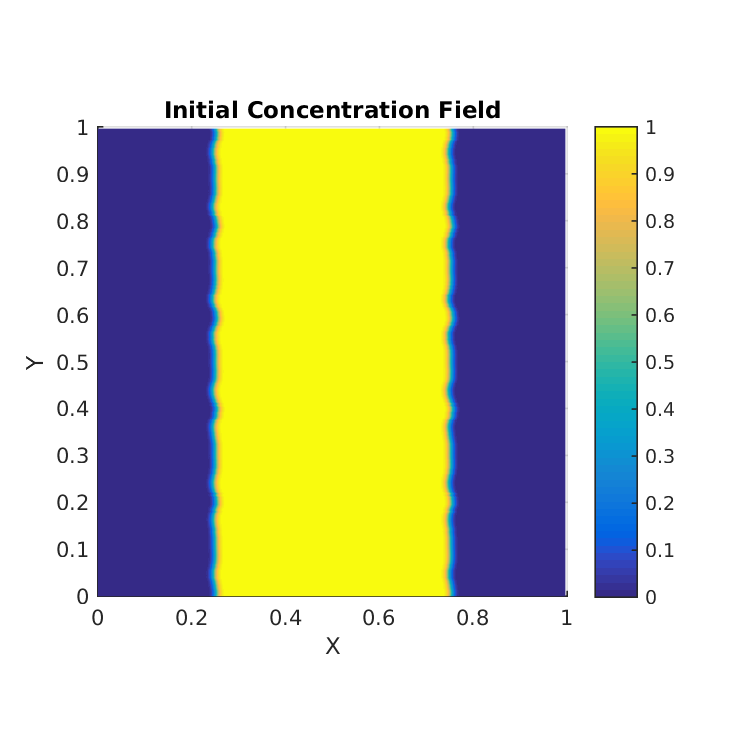
\includegraphics[scale=1.0]{initial_conc.png}
\caption{The initial concentration used for all simulations. There are small pertubations to the otherwise vertical boundary in concentration.}
\label{fig:initial-conc}
\end{figure}

\begin{figure}[!ht]
\centering
\begin{tabular}{c c c}
\includegraphics[scale=0.8]{conc10_1.png} &
\includegraphics[scale=0.8]{conc10_2.png} &
\includegraphics[scale=0.8]{conc10_4.png} &
\end{tabular}
\caption{Concentration plots for R = $1, 2, 2.8$ (top to bottom) at times t $\approx 1, 2, 4$ seconds (left to right).}
\label{fig:conc}
\end{figure}

\item
\end{enumerate}

\subsection{Part 8}
Since our method is using the spectral method for spatial derivatives, the order is very high (dependent on the total number of grid points).
However, because we use a Runge-Kutta 4 explicit scheme for time integration, we are limited to fourth order accuracy in time.
The RK4 scheme has an interesting convergence region (and is slightly larger than the forward Euler scheme).

Setting the viscosity contrast to a large number is probably not good for the current scheme used (explicit mobility).
This is because explicit methods tend to become unstable if the solution variables change ``too much'' during a step.
With a higher viscosity contrast, the mobilities can change more dramatically between time steps, unless much smaller steps are taken.
For a large viscosity contrast, we will probably want to change to an implicit mobility step, where the stream function and vorticity are solved in a simultaneous manner.
This will be more expensive, but should allow for larger viscosity contrasts (though we will still be limited by the RK4 scheme for time integration).

For the time derivative, we can add more stages to the Runga-Kutta scheme (which actually improves the stability properties in addition to the order); the trade off is that more evaluations of spatial derivatives are done per time step.

\clearpage
\appendix
\section{Code}
\lstinputlisting[label=code:solve-vel]{../code/calculate_new_velocity.m}
\lstinputlisting[label=code:solve-vel-opt]{../code/calculate_new_velocity_opt.m}
\lstinputlisting[label=code:solve-conc]{../code/calculate_new_concentration.m}
\lstinputlisting[label=code:solve-conc-opt]{../code/calculate_new_concentration_opt.m}

\end{document}
